% --------------------------------------------------------------
% This is all preamble stuff that you don't have to worry about.
% Head down to where it says "Start here"
% --------------------------------------------------------------
 
 % Template found in: https://gist.github.com/dcernst/1827406
 
\documentclass[12pt]{article}
 
\usepackage[margin=1in]{geometry} 
\usepackage{amsmath,amsthm,amssymb}

\usepackage{physics}

\usepackage{graphicx}
 
\newcommand{\N}{\mathbb{N}}
\newcommand{\Z}{\mathbb{Z}}
 
\newenvironment{theorem}[2][Theorem]{\begin{trivlist}
\item[\hskip \labelsep {\bfseries #1}\hskip \labelsep {\bfseries #2.}]}{\end{trivlist}}
\newenvironment{lemma}[2][Lemma]{\begin{trivlist}
\item[\hskip \labelsep {\bfseries #1}\hskip \labelsep {\bfseries #2.}]}{\end{trivlist}}
\newenvironment{exercise}[2][Exercise]{\begin{trivlist}
\item[\hskip \labelsep {\bfseries #1}\hskip \labelsep {\bfseries #2.}]}{\end{trivlist}}
\newenvironment{problem}[2][Problem]{\begin{trivlist}
\item[\hskip \labelsep {\bfseries #1}\hskip \labelsep {\bfseries #2.}]}{\end{trivlist}}
\newenvironment{question}[2][Question]{\begin{trivlist}
\item[\hskip \labelsep {\bfseries #1}\hskip \labelsep {\bfseries #2.}]}{\end{trivlist}}
\newenvironment{corollary}[2][Corollary]{\begin{trivlist}
\item[\hskip \labelsep {\bfseries #1}\hskip \labelsep {\bfseries #2.}]}{\end{trivlist}}

\usepackage[utf8]{inputenc}

%Algorithm Package
\usepackage[linesnumbered,ruled,vlined]{algorithm2e}

%Math Packages
\usepackage{amsmath}
\usepackage{amssymb}
\usepackage{bm}
\DeclareMathOperator*{\dprime}{\prime \prime}

%Physics Package
\usepackage{physics}

%Allow accentuation marks
\usepackage[utf8]{inputenc}
\usepackage[T1]{fontenc}

%Image packages
\usepackage{graphicx}
\graphicspath{ {Images/} }

%Enumerating lists
\usepackage{enumerate}% http://ctan.org/pkg/enumerate

%Adjust depth of subsections
\setcounter{secnumdepth}{3}

%Adjust depth of table of contents
\setcounter{tocdepth}{3}

%References Packages
%\usepackage{biblatex}
%\addbibresource{references.bib}
\usepackage[bookmarks=true]{hyperref}
\hypersetup{
    hidelinks=true,
    linkcolor=blue,
    filecolor=magenta,      
    urlcolor=cyan,
}

%Commands and packages imported from particle entanglement paper
\usepackage{amsmath}
\usepackage{xcolor}
\usepackage{graphicx}
\usepackage{amssymb}

%\newcommand{\ket}[1]{\vert #1 \rangle}
\newcommand{\eket}[1]{\bigl \vert #1 \bigr \rangle}
\newcommand{\R}{\boldsymbol{R}}
\newcommand{\Rt}{\tilde{\R}}
%\newcommand{\bra}[1]{\langle #1 \vert}
\newcommand{\ebra}[1]{\bigl \langle #1 \bigr \vert}
\newcommand{\eexp}[1]{\bigl \langle #1 \bigr \rangle}
\newcommand{\figref}[1]{Fig.~\ref{#1}}
\renewcommand{\vec}[1]{\boldsymbol{#1}}
\newcommand{\ren}{R\'{e}nyi~}
\newcommand{\rnote}[1]{{\it \textcolor{red}{#1} }}
\newcommand{\Eqref}[1]{Eq.~\eqref{#1}}

%Copied from paper
\usepackage{color}
\usepackage{graphicx}
\usepackage[color=green!60]{todonotes}
\usepackage{physics}
\usepackage{amsthm}
\usepackage{amsmath}
\usepackage{amssymb}
\usepackage{enumerate}
\usepackage{placeins}
\usepackage{booktabs}
\usepackage{dsfont}

%For reference formatting
\usepackage[numbers,sort&compress]{natbib}
\bibliographystyle{nsf_new_url}
 
\begin{document}
 
% --------------------------------------------------------------
%                         Start here
% --------------------------------------------------------------
 
\title{Monte Carlo Methods}%replace X with the appropriate number
\author{Emanuel Casiano-Diaz\\ %replace with your name
PHYS642 - Final Project } %if necessary, replace with your course title
 
\maketitle

Numerical methods are ubiquitously employed in research when an exact evaluation may be out of reach. Such a situation is the evaluation of physical properties in the Ising Model, where the configuration space is of size $2^L$. Monte Carlo simulation are one of the tools that can help bypass this and give reliable results. In this report, a classical Monte Carlo scheme for the square Ising Model is described. It is validated by comparing the with well-known exact solutions of the energy per spin and magnetization per spin. The specific heat per spin is also evaluated at various system sizes and used to obtain an estimate of the ferromagnetic-paramagnetic critical temperature. Finally, the magnetic susceptibility is computed also for various system sizes and the $\nu$ and $\gamma$ critical exponents are obtained to excellent agreement with theoretical results.

\section{Introduction}

Monte Carlo simulation is a powerful computational tool that may provide numerical estimation of problems for which an exact solution does not exist. Solutions are obtained by measuring quantities of interest on a configuration space that changes randomly via a set of updates or moves. Each of these moves is accepted or rejected based on an acceptance ratio that depends on the problem modeled. In this report, a Classical Monte Carlo simulation will be employed to study some quantities of interest in the square Ising Model.

In its simplest form, the Ising Model of magnetism describes a lattice of spins, or magnetic dipoles, that interact with their nearest-neighboring sites, and is subject to periodic boundary conditions, such that spins in the top edge interact with ones at the bottom, and likewise for those on the left and right edges of the square. Mathematically, the model can be formulated by the following Hamiltonian:
%
\begin{equation}
H = -J \sum_{\langle i,j \rangle} \sigma_{i} \sigma_j
\label{eq:ising_hamiltonian}
\end{equation}
%
where $J$ is the interaction strength, $\sigma_i$ gives the value of the spin on site $i$, and the sum is carried over all pairs of nearest-neighbor sites $\langle i,j \rangle$. The probability of measuring a configuration $\lbrace \sigma \rbrace$ is given by the Boltzmann probability distribution:
%
\begin{equation}
P(\lbrace \sigma \rbrace) = \frac{e^{-\beta H}}{\mathcal{Z}}
\end{equation}
\label{eq:probability}
%
where $\mathcal{Z}$ is the partition function. A property that makes this model of interest is the fact that, albeit simple, it still exhibits a phase transition at dimensions $d>2$. Below the critical temperature $T_c$, the system is in the ferromagnetic phase, where spins all spins point to the same direction, wether up or down. Above $T_c$, the spins are randomly oriented, with half of them pointing up, and the other down, on average. As such, there is no net magnetization above $T_c$, but there is below.

This model was solved analytically by Lars Onsager in 1944 \cite{PhysRev.65.117} in the limit of infinitely many fermions. But, a "pen and paper" evaluation of a finite system remains rather difficult due to the fact that there are $2^M$ configurations of spins, where $M$ is the total number of spins. Instead, numerical methods are employed to investigate it, which is where Monte Carlo simulation comes in.

\section{Method}

The Classical Monte Carlo algorithm that will be employed in this report proceeds as follows:

\begin{algorithm}
%\DontPrintSemicolon % Some LaTeX compilers require you to use \dontprintsemicolon    instead
\KwIn{Configuration of spins: $\lbrace \sigma \rbrace$}
\KwOut{New configuration of spins: $\lbrace \sigma_{\rm{new}} \rbrace$}
Set temperature $T$, linear size $L$, bin size, and bins wanted \\
Initialize configuration of spins: $\lbrace \sigma \rbrace$\\
With equal probability, randomly choose a spin \\
Using Eq.~\eqref{eq:ising_hamiltonian}, compute current energy, $E$\\
Using Eq.~\eqref{eq:ising_hamiltonian}, compute energy assuming that chosen spin is flipped, $E_{\rm{new}}$\\
From uniform distribution $U(0,1)$, sample random number r \\
Check, \linebreak
%\renewcommand{\labelenumi}{(\Roman{enumi})}
%\begin{enumerate}[noitemsep,nolistsep]
%\item
If $r < e^{-(E_{\rm{new}}-E)/T}$, flip the chosen spin
\linebreak
%\item 
Else, do not flip the spin \\
%\end{enumerate}
Accumulate data for energy, magnetization, and other estimators every other $L^2$ times that the spin flip update is proposed \\
Write data to file when estimator has been measured a "bin size" amount of times \\
Repeat \textit{Steps 2 to 9} until desired number of bins have been written to file
\caption{Classical Monte Carlo for Square Ising Model}
\label{algo:isingMC}
\end{algorithm}

This algorithm is directly based on the one presented in \cite{giordanoCompPhys}, up to some slight modifications. We start with a configuration of spins $\lbrace \sigma \rbrace$ in an $L \times L$ square lattice. Some parameters are set at the beginning of the simulation, and these are the temperature $T$, the linear size $L$, the bin size, and the bins wanted. The first two are self-explanatory. The bin size sets how many measurements are performed before a quantity is averaged and written to disk. And finally, the bins wanted parameter just sets how many bin-sized-averaged points should be written to disk before stopping the simulation.

A necessary condition that Monte Carlo simulations need to satisfy is that of ergodicity. This means that all possible configurations should be accessible via the set of updates chosen. Moreover, they should be visited in non-periodic fashion. For the case of the Ising lattice, there is really only one update needed that should satisfy ergodicity, and this is the update in which a spin is randomly chosen and flipped. In this update, a random spin is chosen. We then calculate energy difference $E_{\rm{new}}-E$, where the first term is the energy of the configuration assuming that the proposed spin is flip, and the second term is the energy of the current configuration. Both of these energies are computed using the Ising Hamiltonian in Eq.~\eqref{eq:ising_hamiltonian}. Once the energy difference is computed, a Metropolis-Hastings test \cite{doi:10.1063/1.1699114} is used to determine if the spin will actually be flipped or not. This test consists in randomly sampling a uniformly distributed random number $\in [0,1)$ and comparing it with the ratio of probabilities between new and old configurations:
%
\begin{equation}
\frac{P_{\rm{old}}}{P_{\rm{new}}} = e^{-(E_{\rm{new}}-E)/K_BT} \equiv e^{-(E_{\rm{new}}-E)/K_BT}
\end{equation}
%
where we have set $K_B=1$. These equation follows from the fact that spin configurations follow a Boltzmann probability distribution. Note that the test implies that configurations that decrease the energy of the system will always be accepted, since the exponent will become overall positive and the resulting probability ration will alway be larger than the randomly sampled number $r \in [0,1)$.

The data that we will be saving for the purpose of this report are: energy $(E)$, magnetization $(M)$, energy squared $(E^2)$, and magnetization squared $(E^2)$. In step 8 of the algorithm, it is established that measurements will be performed only every other $L^2$ steps. The reason for this is that since the random walk is actually deterministic in nature, as it follows from some pre-determined random number generator, and as such, subsequents configurations will be correlated to each other. By first proposing the spin-flip update $L^2$, we have in principle given the whole system the chance to change, and subsequent measurements should be less correlated. An accessible discussion of correlated sampling can be seen in \cite{2010}. To further decrease inter-sample correlations, we can choose to only write to disk the average of a certain number of measurements. This pre-determined number of measurements is the bin size parameter. Disk space can also be drastically saved by writing these binned averaged. And finally, the algorithm is repeated over and over until the number of desired averaged data points (or bins) are written to file.

\begin{figure}[t]
\begin{center}
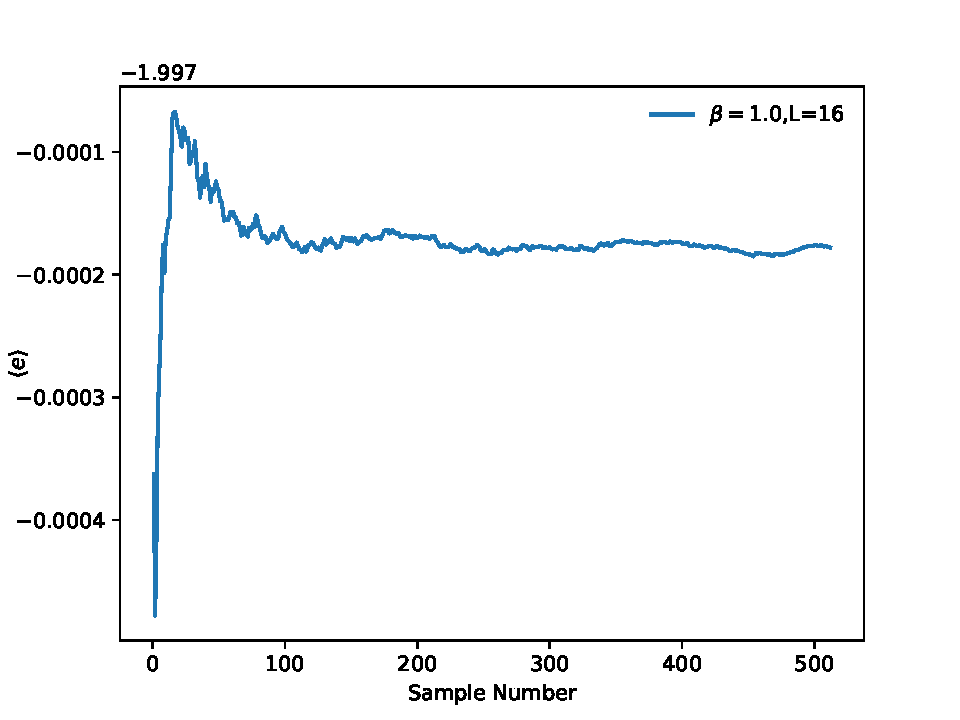
\includegraphics[width=0.7\columnwidth]{../Figures/a_equilibration_beta_1.0}
\end{center}
\caption{Running average of the energy per spin $e \equiv E/L^2$ for a square Ising lattice of linear size $L=16$ at temperature $T=1.0$. The interaction strength has been set to $J=1.0$.The equilibration time is roughly $100$ bins. }
\label{fig:equilibration1}
\end{figure}

\begin{figure}[t]
\begin{center}
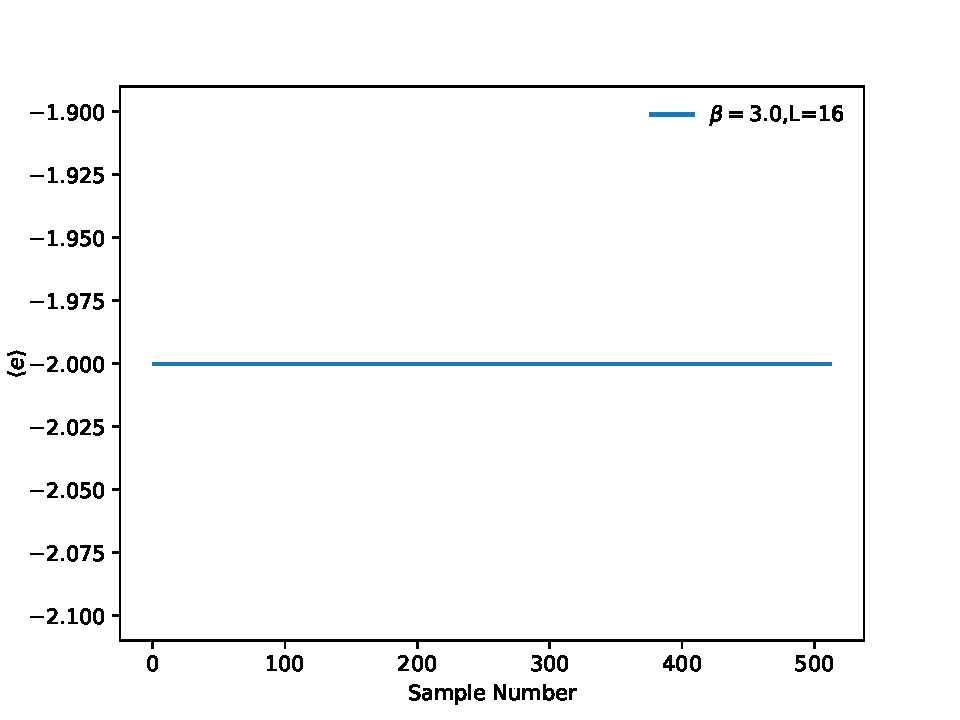
\includegraphics[width=0.7\columnwidth]{../Figures/a_equilibration_beta_3.0}
\end{center}
\caption{Running average of the energy per spin $e \equiv E/L^2$ for a square Ising lattice of linear size $L=16$ at temperature $T=1/3$. The interaction strength has been set to $J=1.0$. Since the lattice was initialized to a configuration with all spins pointing in the same direction, equilibrium configuration, which will be a ferromagnet, is quickly reached.}
\label{fig:equilibration3}
\end{figure}

In the infinitely long time limit, the algorithm should produce the exact values for the desired physical quantities. \figref{fig:equilibration1} and \figref{fig:equilibration3} show a running average of the energy per spin for an $L=16$ system. In \figref{fig:equilibration1}, the temperature is set to $T=1$ and it is seen how the values initially are fluctuating wildly, until they saturate around a horizontal line. The initial period of high fluctuations is known as the equilibration time. For this figure, it is seen that the equilibration time will be roughly $100$ samples. Even though the equilibration time will be different for various parameters, for this report we will assume the same equilibration time for all data. These $100$ first samples will be discarded when computing averages and statistical errors of physical quantities. You might be wondering what is the the reason that \figref{fig:equilibration3} is a straight horizontal line throughout. This figure corresponds to a lower temperature of $T=1/3 (\beta=3)$, which lies in the ferromagnetic phase of the square Ising Model, where all spins point in the same direction. In my implementation of the code, the lattice is initialized with all spins pointing in the same direction. Thus, at low temperatures, the lattice is already initializing at a ferromagnetic configuration, giving the illusion that no equilibration is needed. Randomly initializing the lattice will quickly expose how there will indeed be an associated equilibration time.

In the next section, we will present results for various quantities and compare them with theoretical predictions to test our Monte Carlo implementation.

\section{Results}. 

The first result we will look at is the energy per spin. The total energy E is computed from Eq.~\eqref{eq:ising_hamiltonian}. Energy data is then averaged according to:
%
\begin{equation}
\langle E \rangle = \frac{1}{N_{\rm{samples}}} \sum_{n=1}^{N_{\rm{samples}}} E_n
\end{equation}
%
where $N_{rm{samples}}$ is the number of samples included in the average. The energy per spin can be then computed by dividing the energy between the total number of sites $L^2$. Due to Onsager's legendary calculation, the energy per spin in the asymptotic limit of infinite spins is exactly known:
%
\begin{equation}
e(T) = -J \cot 2K [ 1 + \frac{2}{\pi} (2 \tanh^2 2K - 1)K_1(q)]
\label{eq:e_exact}
\end{equation}
%
where $K\equiv J/K_BT$, $q \equiv 2 \sinh 2K / \cosh^2 2K$, and $K_1(q)$ is the complete elliptic integral of the first kind. \figref{fig:internal_energy} shows the energy per spin as a function of temperature for a square lattice of linear size $L=16$. The Monte Carlo data points fall neatly on top of the Onsager solution, confirming that our Monte Carlo algorithm is working appropriately. Additionally, there is indication that there is a quantum phase transition slightly for a temperature somewhere in the interval $T=[2,3]$.

\begin{figure}[t]
\begin{center}
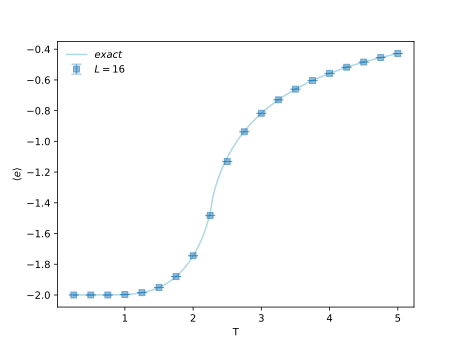
\includegraphics[width=0.7\columnwidth]{../Figures/b_e_per_spin}
\end{center}
\caption{Energy per spin as a function of temperature for a square Ising lattice of linear size $L=16$. Monte Carlo data (points) fall on top the exact solution provided by Onsager (solid line). The data suggests a phase transition between $T=2$ and $T=3$. Error bars are included but are much smaller than the points.}
\label{fig:internal_energy}
\end{figure}

\begin{figure}[h]
\begin{center}
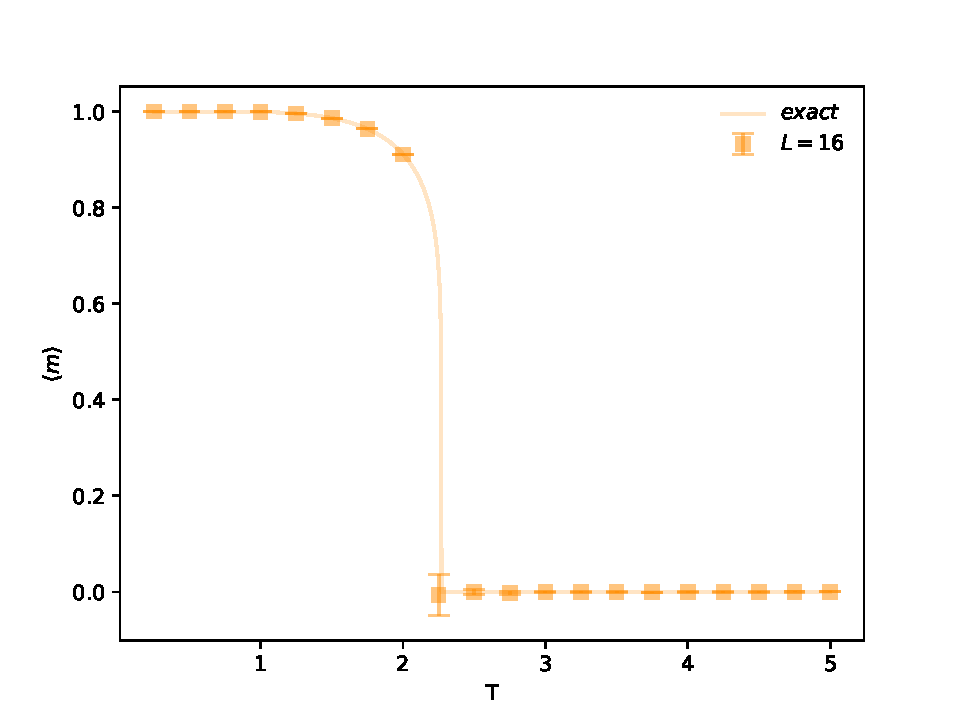
\includegraphics[width=0.7\columnwidth]{../Figures/b_m_per_spin}
\end{center}
\caption{Magnetization per spin as a function of temperature for a square Ising lattice of linear size $L=16$. Monte Carlo data (points) fall on top the exact solution provided by Onsager (solid line). The saturation values at low and high $T$ are indicative of a ferromagnet and a paramagnet, respectively. Error bars are included but are much smaller than the points, except at the value nearest to the phase transition.}
\label{fig:internal_magnetization}
\end{figure}

\begin{figure}[h]
\begin{center}
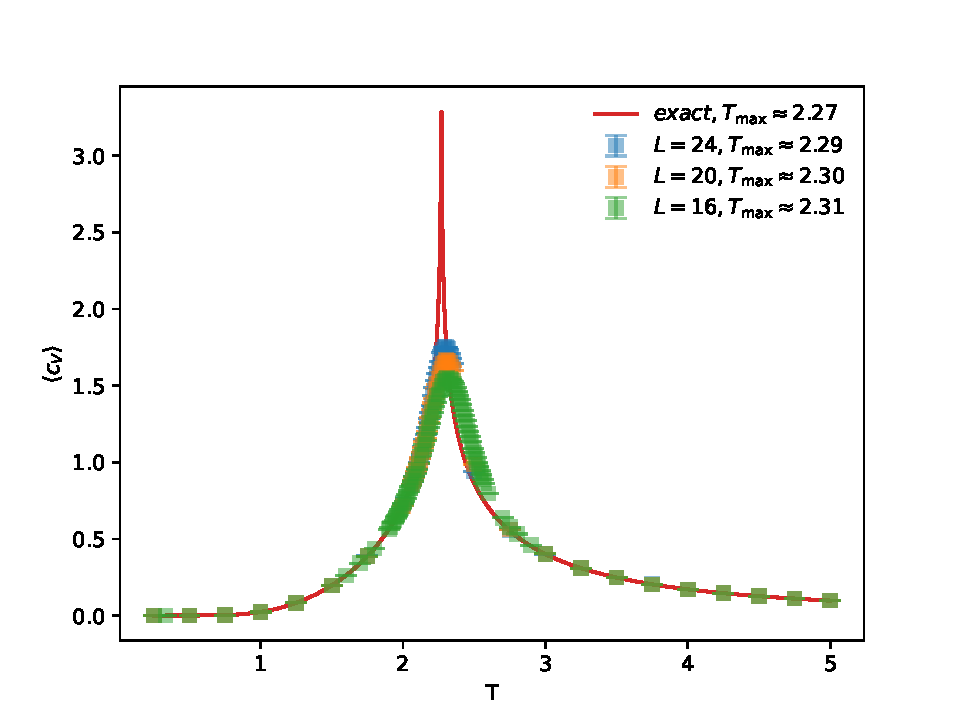
\includegraphics[width=0.7\columnwidth]{../Figures/c_specific_heat}
\end{center}
\caption{Specific heat per spin as a function of temperature. The different colors correspond to various linear sizes. It is seen that theory and simulation match well throughout the temperature range, except at criticality. At the critical point, the sharp peak expected from theory is not matched well by the data, which could be due to finite-size effects. Notice that the peak in the data gets higher with increasing system size.}
\label{fig:cv_vs_T}
\end{figure}

\begin{figure}[h]
\begin{center}
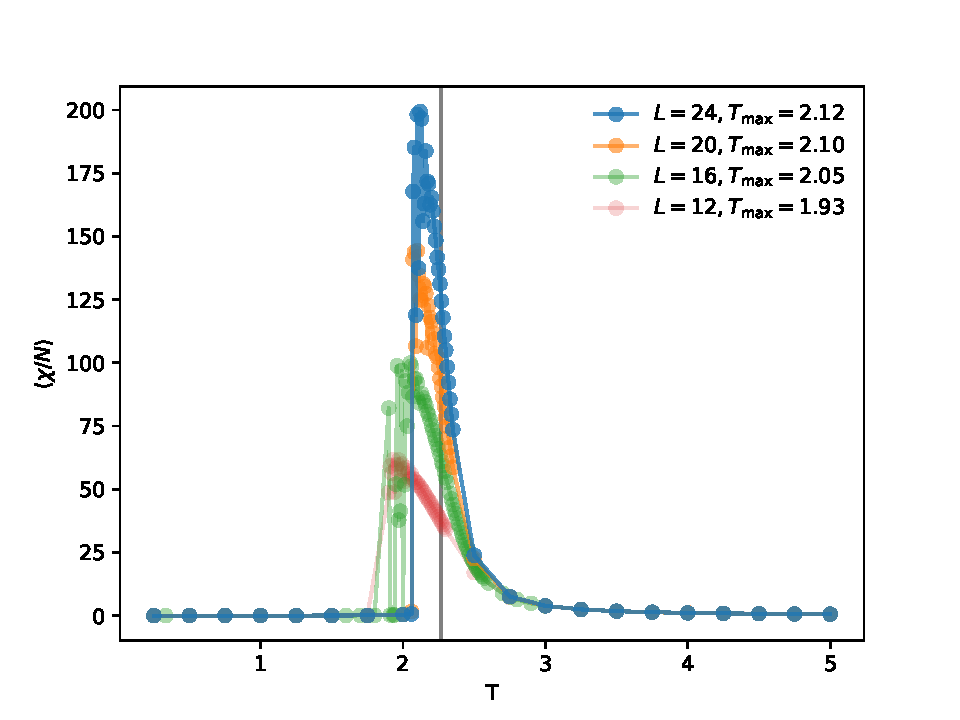
\includegraphics[width=0.7\columnwidth]{../Figures/d_susceptibility}
\end{center}
\caption{Magnetic susceptibility per spin as a function of temperature. The temperature at which the peak occurs moves closer to the exact critical temperature (vertical line) as the system size increases.}
\label{fig:chi}
\end{figure}

\begin{figure}[h]
\begin{center}
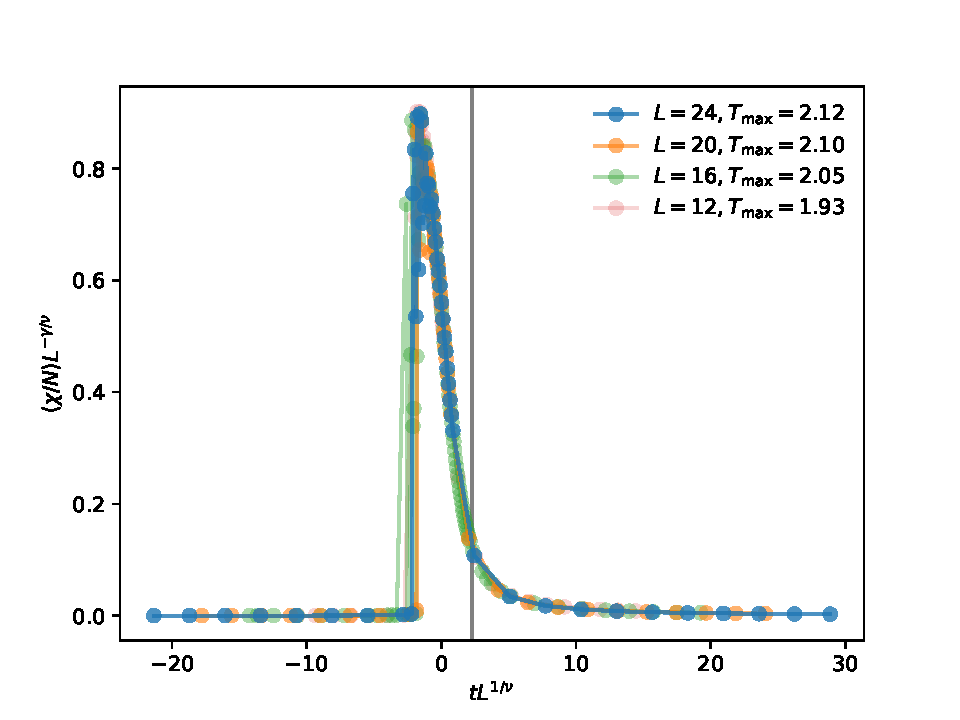
\includegraphics[width=0.7\columnwidth]{../Figures/d_collapse}
\end{center}
\caption{Collapsed susceptibility as a function of T. The exponents $\gamma,\nu$ were tweaked until the data for all system sizes collapsed onto each other. The chosen values that produced the collapsed figure shown were: $\gamma = 1.7$ and $\nu = 1.0$.}
\label{fig:collapse}
\end{figure}

Having successfully estimated the energy per spin for a relatively broad range of temperatures, we now proceed to the same for the magnetization per spin. The total magnetization is computed by: 
%
\begin{equation}
M = \sum_{i=1}^{L^2} \sigma_i
\end{equation}
%
were the sum is carried over all sites. The Monte Carlo estimate is then obtained as:
%
\begin{equation}
\langle M \rangle = \frac{1}{N_{\rm{samples}}} \sum_{n=1}^{N_{\rm{samples}}} M_n
\end{equation}
%
and finally, the magnetization per spin is just obtained by dividing the total average magnetization between the total number of sites: $\langle m \rangle = M/L^2$. The theoretical prediction for the magnetization per spin as function of temperature is:
%
\begin{equation}
m(T) = [1 - \frac{(1-\tanh^2K)^4}{16 \tanh^4K}]^{1/8}
\end{equation}
%
\figref{fig:internal_magnetization} shows the magnetization per spin as a function of temperature for a square lattice of linear size $L=16$. The Monte Carlo data points once again fall neatly on top of the theoretical. Evaluation of limiting cases agrees with the two phases that the model is known to exhibit. In the limit $T\to0$, the magnetization per spin saturates at $1$. This is indicative of a ferromagnet, where all spin point to the same direction. In the limit $T\to\infty$, the spins are completely randomly oriented, with opposing contributions to the magnetization cancelling out, resulting in a magnetization per spin of $0$. Another interesting feature showing up is that the error bars are very small throughout, except near the phase transition, a result most likely resulting from the diverging correlation lengths near criticality.

In our simulation, not only was $\langle E \rangle$ measured and saved to disk, but also the square energy $\langle E^2 \rangle$. The reasoning for this was to easily compute the specific heat via it's fluctuation-dissipation relation:
%
\begin{equation}
C_V = \frac{\langle E^2 \rangle - \langle E \rangle^2}{K_B T^2}
\end{equation}
%
The exact formula for the specific heat per spin is:
%
\begin{equation}
K_B^{-1} c_V(T) = \frac{4}{\pi} (K \coth 2K)^2 \lbrace K_1(q) - E_1(q) - (1-\tanh^2 2K) [\frac{\pi}{2}+(2 \tanh^2 2K - 1)K_1(q)] \rbrace 
\end{equation}
%
where $E_1(q)$ is the complete elliptic integral of the second kind. \figref{fig:cv_vs_T} shows the specific heat per spin as a function of temperature for various system sizes. The Monte Carlo results match the theory well for almost all temperatures, except at at criticality, where the Monte Carlo peak is smaller than the exact one. This could be a finite-size effect, as we can see that for increasing system size, the Monte Carlo peak gets more pronounced. The critical temperature can be estimated by looking at the temperature where the peak is occurring. In the largest system size presented, which is $L=24$, the peak occurs at roughly $T_{\rm{max}}\approx2.29$. Nevertheless, since we have the exact curve plotted using a much more dense $x-axis$, I would feel more comfortable reported the critical temperature as approximately $T_{\rm{c}} \approx 2.27$.

The final quantity we would like to investigate with the data obtained from the Monte Carlo simulation is the magnetic susceptibility. There is also a fluctuation-dissipation relation for this quantity and it is given by:
%
\begin{equation}
\chi = \frac{\langle M^2 \rangle - \langle M \rangle^2}{K_B T}
\end{equation}
%
\figref{fig:chi} shows the magnetic susceptibility per spin as function of temperature for various system sizes.

We would like to some critical exponents from this data, mainly $\gamma$ and $\nu$. To do so, we plot $\langle \chi / N \rangle L^{-\gamma/\nu}$ as a function of $t L^{1/\nu}$, where $t = (T-T_c)/T_c$ is the reduced temperature, and the exact value of the critical temperature, $T_c = 2/\ln (1+\sqrt(2))$ has been chosen. Then, $\nu,\gamma$ can be treated as parameters to be tweaked until the plots corresponding to all the various system sizes collapse onto each other as well as possible. \figref{fig:collapse} illustrates such a collapse happening for values of $\nu = 1.0$ and $\gamma = 1.7$. Comparing these to the exact values, which are $\nu = 1.0$ and $\gamma = 7/4 \approx 1.75$, we see excellent agreement, with even better agreement potentially attainable if not were for the various sources of error, such as finite-size effects and the periodic boundary.

\section{Conclusion}

By employing a classical Monte Carlo algorithm several properties were explored. The energy per spin and magnetization per spin were in almost perfect agreement with Onsager's theoretical formulas, even for our certainly not infinitely sized system of $L=16$. By utilizing fluctuation-dissipation relations, the specific heat and magnetic susceptibility were also studied. The first allowed us to obtain a reasonable approximation of the critical temperature. And the second, allowed us to obtain reasonably good critical exponents $\nu$ and $\gamma$. These results can be further improved in the future by attempting to simulate much larger systems, perhaps by exploiting the perfectly parallel nature of Monte Carlo, since the theoretical predictions shown are in the limit of infinitely many spins.

\section{Code}

The code I developed to generate the data presented, along with instructions on how to run it, can be found in the following public github repository: \url{https://github.com/ecasiano/IsingMonteCarlo}

Due to the total size of the data files, I have not committed them to the repository but can share them upon request.

% Bibliography
\bibliographystyle{unsrt}
\bibliography{references}

%
% --------------------------------------------------------------
%     You don't have to mess with anything below this line.
% --------------------------------------------------------------
 
\end{document}